\documentclass[
  a4paper,
  12pt,
  spanish,
]{scrartcl}

% Párrafos
\setlength{\parindent}{18pt}

%-------------------------------------------------------------------------------
%	PAQUETES
%-------------------------------------------------------------------------------

% Idioma

\usepackage[es-noindentfirst]{babel}

% Citas de texto en línea/bloque

\usepackage[autostyle]{csquotes}

% Matemáticas

\usepackage{amsmath, amsthm, amssymb}
\usepackage{mathtools}
\usepackage{commath}

% Fuentes personalizadas para utilizar con XeLaTeX o LuaLaTeX

\usepackage[no-math]{fontspec}
\setmainfont{Libertinus Serif}
\setsansfont{Libertinus Sans}
\setmonofont{Libertinus Mono}

\usepackage[math-style=TeX]{unicode-math}
\setmathfont{Libertinus Math}

% Configuración de microtype

\defaultfontfeatures{Ligatures=TeX,Numbers=Lining}
\usepackage[activate={true,nocompatibility},final,tracking=true,factor=1100,stretch=10,shrink=10]{microtype}
\SetTracking{encoding={*}, shape=sc}{0}

% Enlaces y colores

\usepackage{hyperref}
\usepackage[dvipsnames]{xcolor}
\definecolor{webgreen}{rgb}{0,0.5,0}
\hypersetup{
  colorlinks=true,
  citecolor=webgreen,
  urlcolor=Maroon,
  linkcolor=RoyalBlue
}

% Otros elementos de página

\usepackage{enumitem}
\setlist[enumerate]{leftmargin=*, itemsep=0pt}
\setlist[itemize]{leftmargin=*, itemsep=0pt}

\usepackage[labelfont=sc]{caption}

% Tikz

\usepackage{tikz}
\usetikzlibrary{babel}
\usepackage{float}

% Código

\usepackage{listings}
\lstset{
	basicstyle=\footnotesize\ttfamily,%
	breaklines=true,%
	captionpos=b,                    % sets the caption-position to bottom
  tabsize=2,	                   % sets default tabsize to 2 spaces
  frame=lines,
  numbers=left,
  stepnumber=1,
  aboveskip=12pt,
  showstringspaces=false,
}
\renewcommand{\lstlistingname}{Listado}

% Bibliografía

\usepackage[sorting=none, style=apa, isbn=true]{biblatex}
\addbibresource{bibliografia.bib}

% Lorem ipsum

\usepackage{blindtext}

% Márgenes
\usepackage[bottom=3.125cm, top=2.5cm, left=4.5cm, right=4.5cm, marginparwidth=70pt]{geometry}

% Fuentes

\usepackage{textcase}

\newfontfamily{\sacshape}{Libertinus Serif}[
  WordSpace={1.8},
  LetterSpace={18.0}
]

\newfontfamily{\slscshape}{Libertinus Serif}[
  WordSpace={1.8},
  LetterSpace={6.0}
]

\DeclareRobustCommand{\spacedallcaps}[1]{{\linespread{1.3}\sacshape\MakeTextUppercase{#1}}}% WordSpace=1.8
\DeclareRobustCommand{\spacedlowsmallcaps}[1]{{\slscshape\MakeTextLowercase{#1}}}% WordSpace=1.8

% Cabeceras de sección

\RedeclareSectionCommands[beforeskip=-3ex,
afterskip=2ex]{section,subsection,subsubsection}
%\addtokomafont{section}{\normalfont\large\spacedallcaps}
%\setkomafont{section}{\normalfont\large\scshape}
\RedeclareSectionCommand[beforeskip=-9ex, font=\normalfont\large\scshape, tocentryformat=\normalfont\scshape]{section}
\addtokomafont{subsection}{\normalfont\normalsize\itshape}
\RedeclareSectionCommand[beforeskip=-6ex,tocentryformat=\normalfont\itshape]{subsection}
\addtokomafont{subsubsection}{\normalfont}
\RedeclareSectionCommand[beforeskip=-4ex]{subsubsection}
\addtokomafont{paragraph}{\normalfont\itshape}

%-------------------------------------------------------------------------------
%	TÍTULO
%-------------------------------------------------------------------------------

\newcommand{\horrule}[1]{\rule{\linewidth}{#1}}

%-------------------------------------------------------------------------------
%	CONTENIDO
%-------------------------------------------------------------------------------

\begin{document}

\begin{titlepage}
  \vspace*{4cm}

  \begin{flushleft}
    \Huge
    \spacedallcaps{Curvas Elípticas en la Criptografía}
    \horrule{2pt}
  \end{flushleft}

  \vspace{2em}

  \begin{flushright}
    \large
    Sofía Almeida Bruno\\
    Antonio Coín Castro\\
    José María Martín Luque\vspace{1em}
  
    \textit{Historia de las Matemáticas}
  
    Grado en Matemáticas
  
    \textsc{Universidad de Granada}\vspace{1em}
  
    \today\vspace{.5em}
  \end{flushright}
\end{titlepage}

\newpage

{\hypersetup{hidelinks}
\tableofcontents
}

\newpage

\section{Introducción}

El objetivo principal de la criptografía es el de la transmisión de información confidencial a través de un canal inseguro.

\section{Curvas elípticas}

Antes de analizar la historia y el papel de las curvas elípticas en el contexto de la criptografía, damos una definición de ellas como objetos matemáticos abstractos.

    Sea $K$ un cuerpo y $\overline{K}$ su clausura algebraica. Una \textit{curva elíptica} sobre $\overline{K}$ es una curva proyectiva no singular $E \subset \mathbb{P}^2(\overline{K})$ definida por una ecuación (afín) de la forma \[ y^2 + a_1xy + a_3y = x^3 +a_2x^2 + a_4x + a_6, \] donde todos los $a_i \in \overline{K}$.
    Cuando la característica de $\overline{K}$ es distinta de $2$ y de $3$, podemos simplificar la ecuación como \[ y^2 = x^3 + Ax + B, \] con $A,B \in \overline{K}$. Una ecuación de esta forma se conoce como \textit{ecuación de Weierstrass}, y en este caso la condición de no singularidad implica que $4A^3 + 27B^2 \neq 0$. Si de hecho los coeficientes $A$ y $B$ están en $K$, decimos que la curva está definida sobre $K$, y nos referimos a ella como \[ E = E(K) = \{ (x, y) \in K \times K : y^2 = x^3 + Ax + B\} \cup \{\mathcal{O}\}, \] donde denotamos por $\mathcal{O}$ al punto en el infinito con coordenadas homogéneas $[0:1:0]$. Notamos que estas curvas son simétricas con respecto al eje de abscisas.
    
\begin{figure}[h]
  \centering
  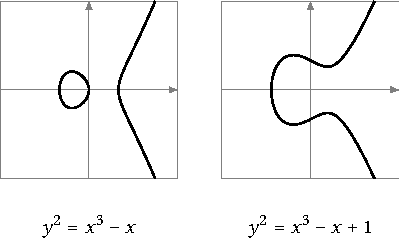
\includegraphics[width=.75\textwidth]{img/ejemplos-curvas}
  \caption{Ejemplos de curvas elípticas sobre $\mathbb{R}$. Basado en \parencite{eichlseder_elliptic_2016}.}
  \label{fig:curva}
\end{figure}

Podemos ver en la figura \ref{fig:parametros} cómo afectan los parámetros $A$ y $B$ a la representación de las curvas elípticas.

\begin{figure}[h]
  \centering
  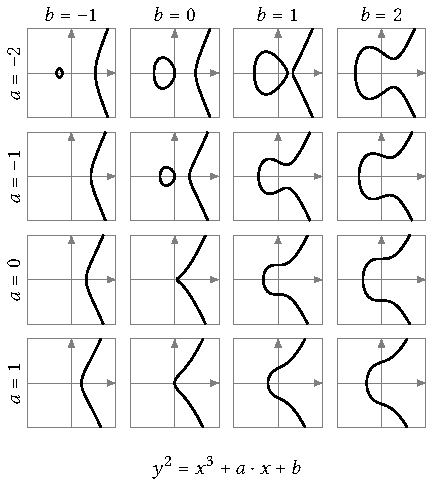
\includegraphics[width=.75\textwidth]{img/parametros-curvas}
  \caption{Ejemplos de curvas elípticas con distintos parámetros \parencite{eichlseder_elliptic_2016}.}
  \label{fig:parametros}
\end{figure}


\subsection{Operación de grupo en curvas elípticas}

Un detalle intersante sobre las curvas elípticas es que se puede definir sobre ellas una operación $+$ de forma que $(E, +)$ sea un grupo abeliano, con elemento identidad el punto $\mathcal{O}$. Para definir esta operación, supondremos por un momento que $K = \mathbb{R}$, y entenderemos que el punto del infinito se encuentra ``al principio'' y ``al final'' del eje de ordenadas. Podemos pensar entonces que dos rectas paralelas se cortan en el punto $\mathcal{O}$, y también que una recta vertical interseca a $E$ en el infinito.

    El procedimiento general es el que sigue. Dados dos puntos $P = (x_1, y_1)$ y $Q = (x_2, y_2)$ con $P,Q \in E$, consideramos la recta que los une y llamamos $R$ a la otra intersección de dicha recta con la curva $E$. Entonces, definimos $P + Q$ como el punto reflejado de $R$ con respecto al eje $X$, al que llamaremos $-R$. Notamos que este procedimiento funciona siempre que la recta considerada corte efectivamente a la curva en otro punto. Discutimos ahora los posibles casos particulares del método.
    
\begin{enumerate}
    \item En primer lugar, si $P=\mathcal{O}$ tendremos que la recta que une $P$ y $Q$ es vertical, luego interseca a la curva en el punto reflejado de $Q$, es decir, $\mathcal{O} + Q = - (-Q) = Q$. Hemos probado de camino que el punto $\mathcal{O}$ actúa como elemento identidad para la operación $+$.
    \item En lo que sigue consideraremos $P, Q \neq \mathcal{O}$. Abordamos primero el caso en el que $x_1 \neq x_2$. Entonces, la recta que une $P$ y $Q$ tiene pendiente \[ m = \frac{y_2 - y_1}{x_2 - x_1}, \] y veremos que corta a la recta en otro punto $R$ que permite aplicar el procedimiento general para calcular $P+Q$.	
    \item Si $Q = P$ con segunda coordenada no nula, no podemos considerar la recta que los une, pero la aproximamos por la recta tangente a $E$ en el punto $P$. Es decir, tomando $y = y(x)$ en la expresión de la curva, podemos derivar implícitamente y obtener la pendiente de la recta tangente: \[ 2yy' = 3x^2 + A \implies m = y_1'(x_1) = \frac{3x_1^2 + A}{2y_1}. \]  Veremos también que la recta tangente corta a la curva en otro punto y podremos aplicar el procedimiento general, computando el valor de $P + P$.
    \item Por último, consideramos el caso $Q = -P$, pues al ser las curvas simétricas respecto al eje $X$ no hay otra posibilidad. Así, la recta que une $P$ y $-P$ es vertical, corta a la curva en $\mathcal{O}$, y por tanto $P + (-P) = -\mathcal{O} = \mathcal{O}$, obteniendo que el elemento inverso de un punto $P$ es su reflejado $-P$. En el caso en que la segunda coordenada sea nula, consideramos de nuevo la recta tangente a $E$ en $P$, y tenemos que sigue siendo vertical y corta a la curva en $\mathcal{O}$, verificándose $P + P = \mathcal{O}$.
\end{enumerate}

\begin{figure}[h]
  \centering
  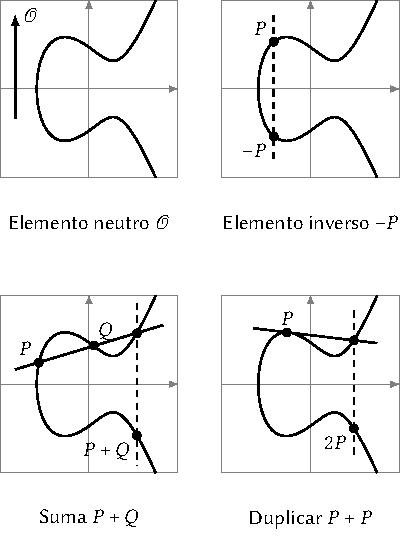
\includegraphics[width=0.65\textwidth]{img/operaciones-curvas}
  \caption{Suma de puntos en curvas elípticas \parencite{eichlseder_elliptic_2016}.}
  \label{fig:operaciones-curvas}
\end{figure}

Veamos ahora cómo calcular el punto de corte de la recta considerada (de pendiente $m$) con la curva $E$, en los casos que no hemos determinado explícitamente la suma de $P+Q$. Podemos escribir la recta como \[ y = m(x - x_1) + y_1, \] y para ver el punto de corte con $E$, sustituimos en su expresión, quedando: \[ (m(x - x_1) + y_1)^2 = x^3 + Ax + B. \] Simplificando esta expresión, obtenemos otra de la forma
\begin{equation}
    \label{eq:corte}
	0 = x^3 - m^2x^2 + bx + c 
\end{equation} 

    Notamos que no es necesario resolver la ecuación cúbica en $x$ para determinar los puntos de corte. Si tenemos un polinomio de la forma $x^3 + ax^2 + bx + c$ y conocemos sus tres raíces $r,s,t$, podemos escribir \[ x^3 + ax^2 + bx + c = (x-r)(x-s)(x-t) = x^3 - (r+s+t)x^2 + dx + e. \] Identificando coeficientes, vemos que $-a = r + s + t$, de donde $t = -a -r -s$. Es decir, si conocemos dos raíces de la expresión, podemos conocer la tercera de forma sencilla.
    
    Volviendo a nuestro caso, conocemos dos soluciones de \eqref{eq:corte}, a saber, $x_1$ y $x_2$ (incluyendo el caso de solución doble $x_1=x_2$). Como $a = -m^2$, podemos calcular la tercera solución de \eqref{eq:corte} fácilmente: \[ x_3 = m^2 - x_1 - x_2. \] Por último, sustituimos en la expresión de la recta para obtener la segunda coordenada del punto de corte, es decir, \[y_3 = m(x_3 - x_1) + y_1, \] y podemos escribir $P+Q = -R$ con $R=(x_3, y_3)$.
    
    Para poder afirmar que $(E, +)$ es un grupo abeliano, falta verificar la conmutatividad y la asociatividad. La primera es obvia o bien de las fórmulas desarrolladas o bien del hecho de que la recta que pasa por $P$ y por $Q$ es la misma que la que pasa por $Q$ y por $P$. La asociatividad es algo menos trivial, pero puede probarse también a partir de las fórmulas para la suma. Una prueba completa puede consultarse en la sección 2.4 de \parencite{elliptic_washington_2008}.
    
    %% Scalar multiplications
    
    
\subsection{Curvas elípticas sobre cuerpos finitos}


%Fórmula concreta, analogía con el caso de R.

% Ejemplo de curva sobre R y curva sobre Z_algo

\section{Evolución de las curvas elípticas en la criptografía}

Un criptosistema es una familia uniparamétrica \(\{S_K\}_{K \in \{K\}}\) de aplicaciones invertibles \[S_K: \{P\} \to \{C\},\] del conjunto de mensajes en claro, \(\{P\}\), al conjunto de mensajes cifrados, \(\{C\}\). 
El parámetro \(K\) se denomina \textit{clave} y el rango de posibles valores que puede tomar \(\{K\}\), \textit{espacio de claves}.

El objetivo a la hora de diseñar un criptosistema \(\{S_K\}\) ha de ser procurar que las operaciones de cifrado y descifrado resulten sencillas pero asegurarse que el análisis criptográfico por parte de terceras personas con el fin de interceptar y descifrar los mensajes cifrados sea lo suficientemente difícil.

\subsection{Criptografía moderna anterior a los años 80}

%Jose.

% - Algoritmo de diffie-hellman, el problema del logaritmo discreto.
% - Tamaño de las claves, número de parámetros, éxito.
% - Problemas existentes.

En los años 70 del siglo pasado se produjeron dos acontecimientos públicos que supusieron grandes avances en el desarrollo de la criptografía moderna \parencite{singh_code_2003}, \parencite{thawte_history_2013}.

En primer lugar, en 1973 la Oficina Nacional de Normas (NBS por sus siglas en inglés, \textit{National Bureau of Standards}), dependiente del Departamento de Comercio del Gobierno Federal de los Estados Unidos, organizó un concurso público para el diseño de un algoritmo de cifrado que pudiese ser adoptado como estándar por parte de dicho Gobierno. 
El 17 de marzo de 1975 se publicó el primer borrador del \textit{Data Encryption Standard} (DES), sistema de cifrado propuesto por un grupo de investigación de IBM.
Tras recibir varias modificaciones con la ayuda de la Agencia de Seguridad Nacional (NSA por sus siglas en inglés, \textit{National Security Agency}) la versión final del algoritmo fue aprobada y publicada por la NBS en noviembre de 1976 y se convirtió en el primer estándar aprobado por una agencia del Gobierno Federal de los Estados Unidos. 
El hecho de que la NSA colaborase en el diseño del algoritmo --modificando la propuesta original de IBM-- suscitó las sospechas de numerosos investigadores, quienes creían que la NSA había introducido una \textit{puerta trasera} en el algoritmo. 
Finalmente, en los años 90 se llegó a la conclusión de que los cambios aportados por la NSA resultaron ser mejoras. %TODO: citation needed
Otra de las críticas que suscitó fue el tamaño elegido para los bloques.
En 2002 fue reemplazado por el algoritmo AES (\textit{Advanced Encryption Standard}), aprobado como estándar por el sucesor de la NBS, el Instituto Nacional de Estándares y Tecnología (NIST por sus siglas en inglés, \textit{National Institute of Standards and Technology}).

\subsubsection{Protocolo de Diffie y Hellman}

El segundo avance significativo, y el que verdaderamente es relevante para nuestro estudio, fue la publicación en 1976 del artículo \textit{New Directions in Cryptography} \parencite{diffie_new_1976} en el que los autores introducen por primera vez la idea del cifrado de clave pública. 
Hasta el momento, todo algoritmo de cifrado necesitaba una clave secreta, compartida únicamente entre el emisor y el receptor. 
La dificultad para llevar a cabo la comunicación cifrada radicaba entonces en la transmisión de dicha clave de forma segura. 
Diffie y Hellman propusieron un criptosistema asimétrico que utiliza una pareja de claves: una pública y otra privada, eliminando así el obstáculo que suponía la transmisión de la clave.

La técnica se basa en la dificultad de calcular logaritmos en un cuerpo finito de \(q\) elementos, denotado \(\mathbb F_q\), siendo \(q\) un número primo. 
Sea \[Y = \alpha^X \mod q, \qquad \text{para } 1 \leq X \leq q - 1,\] donde \(\alpha\) es fijo y es una \textit{raíz primitiva módulo} \(q\), es decir, todo número coprimo con \(q\) es congruente a una potencia de \(\alpha\) módulo \(q\). 
Al elemento \(X\) se le llama \textit{logaritmo de} \(Y\) \textit{de base} \(\alpha\) y \textit{módulo} \(q\): \[X = \log_{\alpha} Y \mod q, \qquad \text{para } 1 \leq X \leq q - 1.\]
El cálculo de \(Y\) a partir de \(X\) es sencillo, necesitándose para ello como mucho \(2 \cdot \log_2 q\) multiplicaciones utilizando el algoritmo de \textit{exponenciación binaria}. Por ejemplo, para \(X = 18\), \[Y = \alpha^{18} = \cramped{(((\alpha^2)^2)^2)^2} \cdot \cramped{\alpha^2}.\]
Sin embargo, la operación inversa de calcular \(X\) a partir de \(Y\) es mucho más compleja, y en ello radica la seguridad de este sistema, como comentaremos más adelante.

A la hora de establecer la comunicación cifrada cada usuario genera un número aleatorio \(X_i\) de forma independiente dentro del rango de enteros \(\{1, 2, \dots, q - 1\}\). 
Dicho número se guarda en secreto, pero se hace público el número \[Y_i = \alpha^{X_i} \mod q\] junto al nombre y dirección que permiten identificar al usuario. 
Cuando los usuarios \(i\) y \(j\) quieren comunicarse de forma segura utilizan la clave \(K_{ij} = \cramped{\alpha^{X_iX_j}} \mod q\). 
El usuario \(i\) obtiene la clave \(K_{ij}\) a partir del número público \(Y_j\) realizando las operaciones \begin{align*}
  K_{ij} &= Y_j^{X_i} \mod q \\
    &= (\alpha^{X_j})^{X_i} \mod q \\
    &= \alpha^{X_jX_i} \mod q \\
    &= \alpha^{X_iX_j} \mod q.
\end{align*}
El usuario \(j\) obtiene la clave de forma análoga, calculando en su caso \[K_{ij} = Y_i^{X_j} \mod q.\]

\subsubsection{Problema de Diffie-Hellman}

Para que una tercera persona pudiese interceptar la comunicación tendría que obtener la clave \(K_{ij}\) a partir de \(Y_i\) e \(Y_j\), para lo que tendría que calcular, por ejemplo, \[K_{ij} = Y_i^{\left(log_{\alpha} Y_j\right)} \mod q.\] 
Este problema se denomina \textit{problema de Diffie-Hellman}. 
En su artículo los autores conjeturan que la resolución de dicho problema es equivalente a resolver el \textit{problema del logaritmo discreto} para alguno de los valores \(Y_i\) o \(Y_j\). Este problema puede enunciarse como: \begin{displayquote}
  Sea \(G\) un grupo y \(\langle g \rangle\) el subgrupo cíclico generado por \(g\). Dado \(g \in G\) y \(a \in \langle g \rangle\), encuentra \(x\) tal que \(g^x = a\).
\end{displayquote}
En 1990 Bert den Boer afirmó que para ciertos primos, el problema de Diffie-Hellman es tan difícil de resolver como el del logaritmo discreto \parencite{goos_diffie-hellman_1990}, tal y como aventuraron Diffie y Hellman 14 años antes.

Un algoritmo se dice de \textit{tiempo polinómico} cuando el tiempo que tarda en ejecutarse está acotado superiormente por un expresión polinómica del tamaño de los datos de entrada de dicho algoritmo \parencite[6]{garey_computers_1979}. Se considera que son estos algoritmos los que pueden calificarse como suficientemente \textit{rápidos} o \textit{eficientes} \parencite[33]{goldreich_computational_2008}.
Por otro lado, los problemas que son tan difíciles de resolver que no existen algoritmos de tiempo polinómico que los resuelvan se conocen como \textit{intratables} \parencite[8]{garey_computers_1979}. 
Dichos problemas son por tanto aquellos que en teoría pueden ser resueltos --dada una cantidad lo suficientemente grande, pero finita, de recursos-- pero que en la práctica el tamaño de este requisito hace que dicha solución no resulte útil.

Hasta ahora no se ha encontrado ningún algoritmo que resuelva el problema del logaritmo discreto en tiempo polinómico, y es de hecho considerado intratable \parencite{rueppel_how_1993}.
El problema de Diffie-Hellman es en consecuencia intratable para ciertos grupos, y en ello radica finalmente la seguridad del protocolo homónimo.


\subsection{Primera aparición de las curvas elípticas en criptografía}
% Enlazar con el apartado anterior

%1984. Algoritmo de Lenstra
En 1984 Hendrik Lenstra propone un nuevo algoritmo de factorización. Su característica más destacada es el uso de las curvas elípticas, ya que es el primer algoritmo criptográfico que las utiliza. A partir de este momento, se comenzó a buscar usos criptográficos para muchas herramientas matemáticas que nunca habían sido utilizadas con este propósito.

%¿Explicar?

%1985. Problema del logaritmo discreto con curvas elípticas. N. Koblitz y V. Miller (de forma independiente)
Al año siguiente, N. Koblitz y V. Miller proponen, de forma independiente, un uso diferente de las curvas elípticas en criptografía. Su idea fue usar un criptosistema como el de Diffie y Hellman utilizando, en vez del grupo multiplicativo sobre un cuerpo finito, el grupo de puntos de una curva elíptica sobre un cuerpo finito. El enunciado del problema es el siguiente:
\begin{displayquote}
  Sea $E$ verificando la ecuación de Weierstrass $y^2+a_1xy+a_3y=x^3+a_2x^2+a_4x+a_6$ con $a_i \in \mathbb{F}_q$. Consideramos $G$ un subgrupo de los puntos de $E$. Dados $P,Q \in G$ encuentra $x \mod{n}$ tal que $Q=xP$. 
\end{displayquote} 
%¿poner ecuación reducida?
Este problema lo denominamos ``problema del logaritmo discreto para curvas elípticas'', aunque no aparezcan logaritmos en él, por su similitud con el problema del logaritmo discreto.

La razón más importante para considerar la criptografía de la curva elíptica fue que no parecía que se pudiera adaptar el ``index calculus'' para usarlo en el grupo de una curva elíptica. El motivo es que en el ``index calculus'' hay que fijar un conjunto de elementos pequeños (factor base) de forma que podamos escribir el resto de elementos de forma eficiente a partir de ellos. Miller [] demostró que si se utiliza la noción más natural de ``pequeño'' se descubre que no hay suficientes puntos para formar una base para el ``index calculus''.

Al comienzo de la criptografía de la curva elíptica unas curvas muy populares eran las definidas en un cuerpo $\mathbb{F}_p$, $p$ primo, que verificaban la ecuación $y^2 = x^3 - x$. El caso ``supersingular'' es aquel en el que se cumple $p \equiv 3 \mod 4$.  Es rápido encontrar un $p$ tal que el grupo tenga un subgrupo grande de orden un primo.

Las curvas supersingulares de característica 2 y 3 tenían otra ventaja: elevar al cuadrado en curvas de característica 2 y al cubo en curvas de característica 3 tardaba un tiempo despreciable.

Pese a que esta elección de parámetros fuera conveniente por los aspectos comentados, los autores que los usaron más adelante se arrepintieron, pues, en 1991, se descubrió que el problema del logaritmo discreto sobre curvas supersingulares es mcho más fácil de resolver que en la mayoría de las curvas. Aunque las curvas supersingulares son muy pocas dentro de todas las curvas elípticas definidas sobre un cuerpo finito, su uso común dio una impresión exagerada sobre su importancia. Así, se pueden usar curvas fáciles de calcular (?)  sin recurrir a las supersingulares.

\subsubsection{Reacciones iniciales}
Durante los años siguientes a la aparición de la criptografía de la curva elíptica la actitud general de los criptógrafos fue aceptación y curiosidad, nadie la consideró una amenaza comercial. Aunque la mayor parte de los investigadores nunca habían estudiado curvas elípticas y no entendían la teoría asociada reaccionaron positivamente a la idea de un nuevo tipo de criptografía basada en ellas. A finales de los años 80, un grupo amplio de matemáticos empezó a trabajar en el tema y los avances que introdujeron se tomaron como un indicador de que la criptografía de clave pública pronto estaría lista.

Es en este periodo cuando tres profesores de la universidad de Waterloo crearon una compañía que desarrolló e impulsó la criptografía de la curva elíptica. 


\subsubsection{Algoritmo de firma}

La mayor parte de los algoritmos que utilizaban las curvas elípticas consistían en adaptar los ya existentes para este grupo, no aprovechaban la estructura específica de las curvas elípticas.

% TODO: contar aparición de DSA...NSA
Destacamos la adapación del algoritmo DSA, ya que fue un proceso complicado. En ECDSA (\textit{Elliptic Curve Digital Signature Algorithm}) suponemos que Alice quiere firmar un mensaje con su clave privada ($k_A$) y Bob quiere validar la firma usando la clave pública de Alice ($K_A$). La única que debería poder emitir firmas válidas es Alice, y estas deberían poder ser verificadas por cualquiera que conozca su clave pública.

Alice y Bob usarán los mismos parámetros. Necesitan estar trabajando sobre la misma curva elíptica definida sobre un cuerpo $\mathbb{F}_q$ que contiene un subgrupo $G$ de orden primo ($n$) con generador $P$.

ECDSA no trabaja sobre el mensaje, sino sobre una función \textit{hash} del mismo, que deberá ser truncada si su longitud supera $n$ (el orden del subgrupo).

Alice comienza \textit{generando sus claves}. Para ello, elige aleatoriamente un entero $x$ en el intervalo $[0,n-1]$ y calcula $Q=xP$. La clave pública de Alice será $K_A=Q$ y la privada $k_A=x$.

Para \textit{firmar el mensaje} conociendo su valor \textit{hash} H, Alice:

\begin{enumerate}
\item Elige aleatoriamente un entero $z$ en el intervalo $[1,n-1]$.
\item Calcula el punto $zP =(x_1,x_2)$.
\item Calcula el número $r \equiv x_1 \mod n$.
\item Si $r=0$, elige otro número $z$ y vuelve a empezar.
\item Calcula $s=z^{-1}(H+rk_A)\mod n$. \label{en:s}
\item Si $s=0$, elige otro valor $z$ y lo vuelve a intentar.
\end{enumerate}

La pareja $(r, s)$ es la firma del mensaje. Para obtenerla se generó un valor aleatorio $z$ que será escondido gracias a la multiplicación de puntos, a continuación, en el paso \ref{en:s}, $r$ es ligado al mensaje \textit{hash}. Para calcular el inverso de $z$ módulo $n$ es necesario que $n$ sea un número primo. Si el subgrupo no tiene orden primo, no podremos usar este algoritmo.

Para verificar la firma sobre un mensaje Bob necesita: la clave pública de Alice ($K_A$), el valor \textit{hash} del mensaje ($H$) y su firma ($(r,s)$). Una vez conozca estos tres valores puede comenzar la verificación, para ello:

\begin{enumerate}
\item Calcula $u_1 \equiv s^{-1}H \mod n$ y $u_2 \equiv s^{-1}r \mod n$.
\item Calcula $u_1P + u_2 K_A = (x_0, y_0)$.
\item La firma será válida si, y solo si, $r \equiv x_0 \mod n$.
\end{enumerate}

Si Alice generó su firma correctamente, entonces $u_1P+u_2K_A=(u_1+k_Au_2)P=zP$ porque $z \equiv s^{-1}(H+k_Ar) \mod n$ y $r \equiv x_0 \mod n$.

%Tamaño de las claves, número de parámetros, éxito.

%Problemas existentes

\subsection{<<Paradigm shift>>}

%Sofi.

%Pairing-based cryptography

\subsection{Estado actual y algoritmos utilizados}

%Antonio.

\section{Usos futuros}

%Jose.

%Quantum. https://www.esat.kuleuven.be/cosic/elliptic-curves-are-quantum-dead-long-live-elliptic-curves/

%-------------------------------------------------------------------------------
%	BIBLIOGRAFÍA
%-------------------------------------------------------------------------------

\newpage
\printbibliography

\end{document}
